\documentclass[pdf, aspectratio=169, 12pt]{beamer}
\usepackage[]{hyperref, graphicx, siunitx, lmodern, tikz, booktabs, physics}
\usepackage[mode=buildnew]{standalone}
\usepackage{pdfpc-commands}

\usetheme[sols]{Python}

\graphicspath{ {Images/} }

\sisetup{per-mode=symbol}
\usetikzlibrary{calc, patterns, decorations.markings, decorations.pathmorphing, shapes}

%Preamble
\title{Bring your coins!}
\author{Jed Rembold}
\date{February 5, 2020}

\begin{document}

\begin{frame}{Announcements}
	\begin{itemize}
		\item Homework
			\begin{itemize}
				\item Homework 1 all graded! Check GitHub!
				\item Homework 2 due on Friday night
				\item After today should have everything you need to complete the assignment
			\end{itemize}
		\item Polling: \url{rembold-class.ddns.net}
	\end{itemize}
\end{frame}

\begin{frame}{Homework Comments}
	\begin{itemize}
		\item All HW1 has been graded. Comments and scores uploaded to GitHub.
		\item Most common issues:
			\begin{itemize}
				\item Not following instructions about what to print (usually not that big of a deal when I check myself, but can mask other errors)
				\item Having ``holes'' in blocks of conditional statements.
				\item Comments are optional\ldots until they cost you points.
				\item Just change the ``Assignment status:'' line in the README file please! Not the entire filename!
			\end{itemize}
		\item That said, most people did quite well
	\end{itemize}
\end{frame}

\begin{frame}[fragile]{Review Question}
	Suppose you have the string: \pyi{x = "consternation"} and you'd like to just extract and print the word \pyi{"nation"}. Which expression below will \alert{not} give you the string \pyi{"nation"}?

	\begin{poll}
	\item \pyi{x[7:len(x)]}
	\item \pyi{x[7:]}
	\item \pyi{x[-6:len(x)]}
	\item \pyi{x[-6:-1]}
	\end{poll}
	\exsol{\pyi{x[-6:-1]}}
\end{frame}

\begin{frame}[fragile]{Can't change a string's colors}
	\begin{itemize}
		\item Strings are what we call \alert{immutable}: they can not be modified in place
		\item You can ``look'' at different parts of the string, but you can not ``change'' those parts
			\begin{itemize}
				\item Phased differently, you can't reassign the various pieces of a string
			\end{itemize}
			
			\begin{pythoncode}
				s = "Cats!"

				s[0] = "R"			# This will error!!
			\end{pythoncode}
		\item You can of course still reassign \pyi{s} to some new string object
			\begin{pythoncode}
				s = "R" + s[1:]
			\end{pythoncode}
	\end{itemize}
\end{frame}

\begin{frame}{Enter the Arcade}
	\vspace{5mm}
	\begin{itemize}
		\item There comes a time when reading and entering text on a terminal doesn't cut it.
			\begin{itemize}
				\item Maybe you need more complicated input
				\item Maybe you need a more complicated interface than pure text can manage
				\item Maybe you have output that can not be shown in text
			\end{itemize}
		\item Standard Python really only deals with a terminal interface
		\item Lots of outside ``extensions'' give Python a more visual input/output
			\begin{itemize}[<+->]
				\item Turtle
				\item Matplotlib
				\item Tkinter/Graphics.py
				\item PyQt
				\item PyGame
				\item \alert{Arcade}
			\end{itemize}
	\end{itemize}
\end{frame}

\begin{frame}[fragile]{Setup Costs}
	\vspace{5mm}
	\begin{itemize}
		\item Arcade is not part of the Python ``standard library''
			\begin{itemize}
				\item Also doesn't come packaged by default with Anaconda
				\item You will need to install it separately, which we will cover in lab today
			\end{itemize}
		\item Will need to \pyi{import} it at the top of your file to use its special commands
			\begin{itemize}
				\item Importing is how you gain the powers of ``outside'' libraries in Python
				\item We'll discuss in more detail in Ch 4 in terms of how to import your own files and break up your code.
				\item After import, will always have that library's name at the start of every command from that library:
					\begin{pythoncode}
						import fish

						fish.make_a_fish()
						fish.make_fish_swim()
					\end{pythoncode}
			\end{itemize}
	\end{itemize}
\end{frame}

\begin{frame}[fragile]{The Basics}
	\begin{itemize}
		\item At its simplest, \pyi{arcade} does the following:
			\begin{itemize}
				\item Open a window:
					\begin{pythoncode}
						arcade.open_window(<width>, <height>, <name>)
					\end{pythoncode}
				\item Draw things to the window:
					\begin{pythoncode}
						arcade.draw_circle_filled(0,0,10, arcade.color.RED)
					\end{pythoncode}
				\item Keep the window open so we can see it:
					\begin{pythoncode}
						arcade.run()
					\end{pythoncode}
			\end{itemize}
	\end{itemize}
\end{frame}

\begin{frame}[fragile]{What to draw?}
	\begin{itemize}
		\item You have a wide variety of primitive objects you can draw
			\begin{itemize}
				\item Circles
				\item Rectangles
				\item Lines
				\item Arcs
				\item Polygons
			\end{itemize}
		\item Most have filled/outline options available
			\begin{pythoncode}
				arcade.draw_circle_filled()
				arcade.draw_circle_outline()
			\end{pythoncode}
		\item All start with \pyi{arcade.draw_<what to draw>}
	\end{itemize}
\end{frame}

\begin{frame}{Where to draw?}
	\begin{columns}
		\column{0.5\textwidth}
		\begin{itemize}
			\item Uses a standard x-y coordinate system like in math
			\item Only uses the first quadrant, so everything positive
			\item (0,0) is in the lower left corner
				\begin{itemize}
					\item This is different from many computer graphics programs, which put (0,0) in the upper left corner.
				\end{itemize}
		\end{itemize}
		\column{0.5\textwidth}
		\begin{center}
			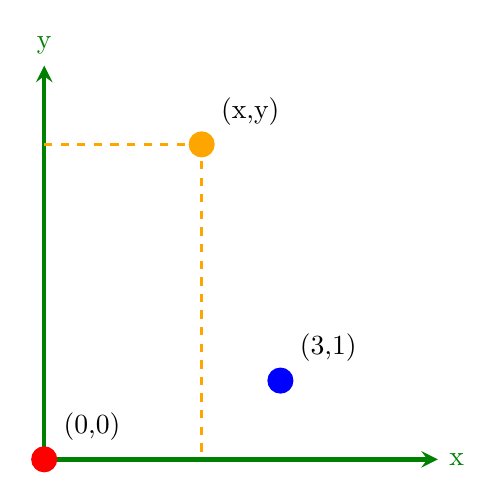
\begin{tikzpicture}
				\draw[Green, ultra thick, -stealth] (0,0) -- +(5,0) node[right] {x};
				\draw[Green, ultra thick, -stealth] (0,0) -- +(0,5) node[above] {y};
				\node[fill=Red, circle, label={above right:(0,0)}] at (0,0) {};
				\node[fill=Blue, circle, label={above right:(3,1)}] at (3,1) {};
				\node[fill=Orange, circle, label={above right:(x,y)}] at (2,4) {};
				\draw[Orange, very thick, dashed] (2,4) -- +(-2,0) 
												  (2,4) -- +(0,-4);
			\end{tikzpicture}
		\end{center}
	\end{columns}
\end{frame}

\begin{frame}[fragile]{How to draw?}
	\begin{itemize}
		\item All drawing commands you make must be between two extra commands:
			\begin{pythoncode}
				arcade.start_render()

				<draw all your stuff here!>

				arcade.finish_render()
			\end{pythoncode}
		\item If you want to change the default background of your window, it goes before the \pyi{arcade.start_render()}:
			\begin{pythoncode}
				arcade.set_background_color()
			\end{pythoncode}
	\end{itemize}
\end{frame}

\begin{frame}[fragile]{I demand rainbows}
	\vspace{8mm}
	You can pick colors in a variety of ways:
	\begin{itemize}
		\item Using arcade's \link{http://arcade.academy/arcade.color.html}{built in colors} (there are 1000. Go wild!)
			\begin{pythoncode}
				arcade.color.ANTIQUE_FUCHSIA
			\end{pythoncode}
		\item Using arcade's \link{http://arcade.academy/arcade.csscolor.html}{css colors} (only 147 here!)
			\begin{pythoncode}
				arcade.csscolor.SILVER
			\end{pythoncode}
		\item Using RGB codes (16.7 million possibilities here\ldots)
			\begin{itemize}
				\item 0 is the min, 255 the max
				\item Come as a set of 3 (or 4) with comma's separating them
				\item Fourth option will give transparency
				\footnotesize
				\begin{pythoncode}
					red = (255,0,0)
					trans_dark_green = (0,100,0,100)
				\end{pythoncode}
			\end{itemize}
	\end{itemize}
\end{frame}


\end{document}

